\documentclass[letterpaper]{article}

\usepackage{natbib,paper/alifeconf}  %% The order is important
\usepackage{amsmath}
\usepackage{hyperref}

\newcommand{\reduceCaptionPadding}{\setlength{\belowcaptionskip}{-10pt}}

\renewcommand\floatpagefraction{.9}
\renewcommand\dblfloatpagefraction{.9} % for two column documents
\renewcommand\topfraction{.9}
\renewcommand\dbltopfraction{.9} % for two column documents
\renewcommand\bottomfraction{.9}
\renewcommand\textfraction{.1}   

% *****************
%  Requirements:
% *****************
%
% - All pages sized consistently at 8.5 x 11 inches (US letter size).
% - PDF length <= 8 pages for full papers, <=2 pages for extended
%    abstracts.
% - Abstract length <= 250 words.
% - No visible crop marks.
% - Images at no greater than 300 dpi, scaled at 100%.
% - Embedded open type fonts only.
% - All layers flattened.
% - No attachments.
% - All desired links active in the files.

% Note that the PDF file must not exceed 5 MB if it is to be indexed
% by Google Scholar. Additional information about Google Scholar
% can be found here:
% http://www.google.com/intl/en/scholar/inclusion.html.


% If your system does not generate letter format documents by default,
% you can use the following workflow:
% latex example
% bibtex example
% latex example ; latex example
% dvips -o example.ps -t letterSize example.dvi
% ps2pdf example.ps example.pdf


% For pdflatex users:
% The alifeconf style file loads the "graphicx" package, and
% this may lead some users of pdflatex to experience problems.
% These can be fixed by editing the alifeconf.sty file to specify:
% \usepackage[pdftex]{graphicx}
%   instead of
% \usepackage{graphicx}.
% The PDF output generated by pdflatex should match the required
% specifications and obviously the dvips and ps2pdf steps become
% unnecessary.


% Note:  Some laser printers have a serious problem printing TeX
% output. The use of ps type I fonts should avoid this problem.

%%%%%%%%%%%%%%%%%%%%%%%%%%%%%%%%%%%%%%%%%%%%%%%%%%%%%%%%
% ======================== TODO ========================
% --- CITATIONS ---
% - [ ] Add in avida-related citations
% --- TEXT ---
% - [ ] make sure we mention difference in how we pull out representative lineages in avida vs. benchmark problems
% - [ ] Decide/work out task vs. function for boolean logic computations
%       - no-task to minimal environment
% - [ ] Switch - 'expected' to 'expects' => smooth out tense, make consistent
% - [ ] Include more experiment config description in methods: updates, mutations(?), etc
%%%%%%%%%%%%%%%%%%%%%%%%%%%%%%%%%%%%%%%%%%%%%%%%%%%%%%%%

% Alternative titles:
%  - A Suite of Metrics for Understanding Evolutionary Dynamics/Histories
%  - Quantifying Evolutionary Histories 
%  - A Suite of Metrics for Quantifying Evolutionary Histories
\title{Interpreting the Tape of Life: Ancestry-based Metrics Provide Insights and Intuition about Evolutionary Dynamics}
\author{Emily Dolson$^{1,2,3}$, Alexander Lalejini$^{1,2, 3}$, Steven Jorgensen$^{1,2}$ \and Charles Ofria$^{1,2, 3}$ \\
\mbox{}\\
$^1$BEACON Center for the Study of Evolution in Action, Michigan State University, East Lansing, MI, 48824 \\
$^2$Department of Computer Science and Engineering, Michigan State University, East Lansing, MI, 48824 \\
$^3$Ecology, Evolutionary Biology, and Behavior Program, Michigan State University, East Lansing, MI, 48824 \\
dolsonem@msu.edu} % email of corresponding author

% For several authors from the same institution use the same number to
% refer to one address.
%
% If the names do not fit well on one line use
%         Author 1, Author 2 ... \\ {\Large\bf Author n} ...\\ ...
%
% If the title and author information do not fit in the area
% allocated, place \setlength\titlebox{<new height>} after the
% \documentclass line where <new height> is 2.25in



\begin{document}
\maketitle

\begin{abstract}
Fine-scale evolutionary dynamics can be challenging to tease out when focused on the broad brush strokes of whole populations over long time spans. We propose a suite of diagnostic metrics that operate on lineages and phylogenies in digital evolution experiments with the aim of improving our capacity to quantitatively explore the nuances of evolutionary histories in digital evolution experiments. We present three types of lineage measurements: lineage length, mutation accumulation, and phenotypic volatility. Additionally, we suggest the adoption of four phylogeny measurements from biology: phylogenetic richness, phylogenetic divergence, phylogenetic regularity, and depth of the most-recent common ancestor. 
%OLD TEXT: We demonstrate the use of each metric on a set of two-dimensional, real-valued optimization problems under a range of mutation rates and selection strengths, confirming our intuitions about what they can tell us about evolutionary dynamics. 
% @AML: A first pass at trying to shove Avida into the old last sentence:
We examine the behavior of these metrics in two well-studied computational contexts: (1) a set of two-dimensional, real-valued optimization problems under a range of mutation rates and selection strengths, and (2) a set of qualitatively different environments in the Avida Digital Evolution Platform.  These results confirm our intuition about how these metrics respond to various evolutionary conditions and indicate their broad value.
 
\end{abstract}

\section{Introduction}

Evolution is a collective effect of many smaller events such as replication, variation, and competition that occur on a fine-grained temporal scale. While evolution's emergent nature can be fascinating, it also presents challenges to studying the short-term mechanisms that, in aggregate, govern long-term results. In computational evolutionary systems, we can theoretically collect data to help untangle these mechanisms. In practice, however, the sheer number of constituent events produce an overwhelming quantity of data.
In response, we have developed a standardized suite of diagnostic metrics to summarize short-term evolutionary dynamics within a population by measuring lineages and phylogenies. Here, we describe these metrics and provide experimental results to develop an intuition for what they can tell us about evolution.

A lineage describes a continuous line of descent, linking parents and offspring in an unbroken chain from an original ancestor.
A complete lineage can provide a post-hoc, step-by-step guide to the evolution of an extant organism where each step involves replication and inherited variation. Indeed, lineage analyses are a powerful tool for disentangling evolutionary dynamics in both natural and digital systems; digital systems, however, allow for perfect lineage tracking at a level of granularity that is impossible in modern wet lab experiments.  These data allow us to replay the tape of life in precise detail and to tease apart the evolutionary recipe for any phenomenon we are interested in~\citep{mcphee_using_2016}. 
In one notable example, Lenski \textit{et al.} used the lineage of an evolved digital organism in Avida to tease apart, step by step, how a complex feature (the capacity to perform the equals logical operation) emerged~\citep{lenski_evolutionary_2003}. 

Yet, tracking the full details of a single lineage, much less a population of lineages, can be computationally expensive and will inevitably generate an unwieldy amount of data that can be challenging to visualize or interpret~\citep{mcphee_visualizing_2016}.
Summary statistics can help alleviate these issues by enabling the user to focus on aggregate trends across a population rather than needing to examine each individual's lineage.
The question is how to effectively summarize a path through fitness space. One useful abstraction is to treat the path as a sequence of states. Here, we use phenotypes and genotypes as the states in the sequence, but we could just as easily use some other descriptor of the lineage's position in the fitness landscape at a given point in time.
With this abstraction in hand, a few metrics are easily formalized: the number of unique states, the number of transitions between states, and the amount of time spent in each state.
Additionally, we may care about how the transitions between states happened. What mutations led to them? Were those mutations beneficial, deleterious, or neutral at the time? These mutations are particularly notable because they did not simply appear briefly, but stood the test of time, leaving descendants in the final population.
%@CAO: Does the sentence I added above make sense?  My point being that these aren't just a random sampling of possible mutations that we are considering.  It's almost worth an extra sentence to point out that any deleterious mutations on the lineage are of special interest since they made it into the lineage despite being actively selected against.
% @AML: I think so. My interpretation: all mutations (beneficial, deleterious, neutral, etc., etc.) that appear on a lineage of an extant individual are particularly notable. 
%Here, we choose a subset of these metrics that we expect will be broadly useful to explore further.
%@ELD: I agree. It's also nice to emphasize in light of deleterious mutations being the most interesting part of our results.
Here, we explore a subset of these metrics that we expect will be broadly useful.

Whereas a lineage recounts the evolutionary history of a single individual, a phylogeny details the evolutionary history of an entire population. Measurements that summarize phylogenies can provide useful insight into population-level evolutionary dynamics, such as diversification and co-existence among different clades. A variety of useful phylogeny measurements have already been developed by biologists~\citep{tucker_guide_2017}. These measurements tend to treat the phylogeny as a graph and make calculations about its topology. Tucker \textit{et al.} group them into three broad categories: assessments of the quantity of evolutionary history represented by a population, assessments of the amount of divergence within that evolutionary history, and assessments of the topological regularity of the phylogenetic tree. Such measurements can help quantify the behavior of the population as a whole, providing insight into interactions between its members. Thus, they are useful indicators of the presence of various types of eco-evolutionary dynamics.

Here, we present three types of lineage measurements and suggest adopting four phylogeny measurements from biology; these are lineage length, mutation accumulation, phenotypic volatility, depth of the most-recent common ancestor, phylogenetic richness, phylogenetic divergence, and phylogenetic regularity.
For each metric, we discuss its application and our expectation for what it can tell us about evolution. 
% OLD TEXT: We evaluate our intuition on a set of two-dimensional, real-valued optimization problems under a range of mutation rates and selection strengths. 
We evaluate our intuition in two computational contexts: first, on a set of two-dimensional, real-valued optimization problems under a range of mutation rates and selection strengths and, second, on four qualitatively different environments in the Avida Digital Evolution Platform 
% @AML: We probably want to mention what types of Avida environments we use...
(the minimal environment, the logic-9 environment with unlimited resources, the logic-9 with limited resources, and a simple changing environment).
For simplicity, we restrict our attention to asexually reproducing populations; however, we suggest how these metrics can be extended to sexual populations. 

In addition to demonstrating a range of metrics that are %immediately applicable and
useful to digital evolution research, we intend for this work to begin a conversation within the %computational evolution
artificial life community about how we quantify, interpret, and compare observed evolutionary histories. There have been extensive efforts to improve our ability to represent and visualize both lineages and phylogenies~\citep{standish_visualising_2002,burlacu_visualization_2013, mcphee_using_2016,mcphee_visualizing_2016, lalejini_evolutionary_2016}, which are indispensable for building intuitions and qualitatively understanding the dynamics embedded in a population's evolutionary history. However, we are unaware of efforts to formalize a suite of quantitative lineage and phylogeny-based metrics for computational evolution. %Indeed, .... % people have done stuff with lineages
% @CAO: For the moment I commented the "Indeed" out since I'm not sure where it's going; think the current version is a fine place to stop, though I also agree that some of the points below would be good to include if we can.
% @AML: We should have room now!
Lineage and phylogeny-based analyses in artificial life are often a component of a larger set of experiment-specific analyses or are limited to qualitative descriptions and/or visualizations. 
Well-defined metrics not only provide valuable tools for teasing apart evolutionary dynamic, they also allow us to move away from exclusively qualitative descriptions of results toward a deeper quantitative understanding, which, in turn, facilitates rigorous statistical analyses and hypothesis testing as well as the ability to more easily compare evolutionary dynamics across different digital evolution systems.
% - often a component of a larger experiment-specific analysis or limited to qualitative descriptions/visualizations
% - well-defined metrics not only provide valuable tools for teasing apart evolutionary dynamics, they also facilitate allow us to move away from exclusively qualitative descriptions/understandings of results ==> better quantitative understanding/statistics ==> better hypothesis testing
% - facilitate comparisons among systems. 
% - Something about activity metrics?

\section{Metrics}

Code for all of our metrics is open source and available in the Empirical library (\url{https://github.com/devosoft/Empirical}). Empirical is a C++ library built to facilitate writing efficient and easily sharable scientific software. %To simplify including useful features with minimal overhead, 
Empirical is a header-only library, so adding these metrics to an existing project has minimal overhead.
% [QUESTION] @AML: Is it actually true that someone could include these metrics with minimal effort? How much of Empirical would it impose on the user? Just the systematics manager? 
%@ELD: They should just need the systematics manager. And they might need to hook up a couple of data collection signals.

\subsection{Lineage Metrics}

\begin{figure*}[t]
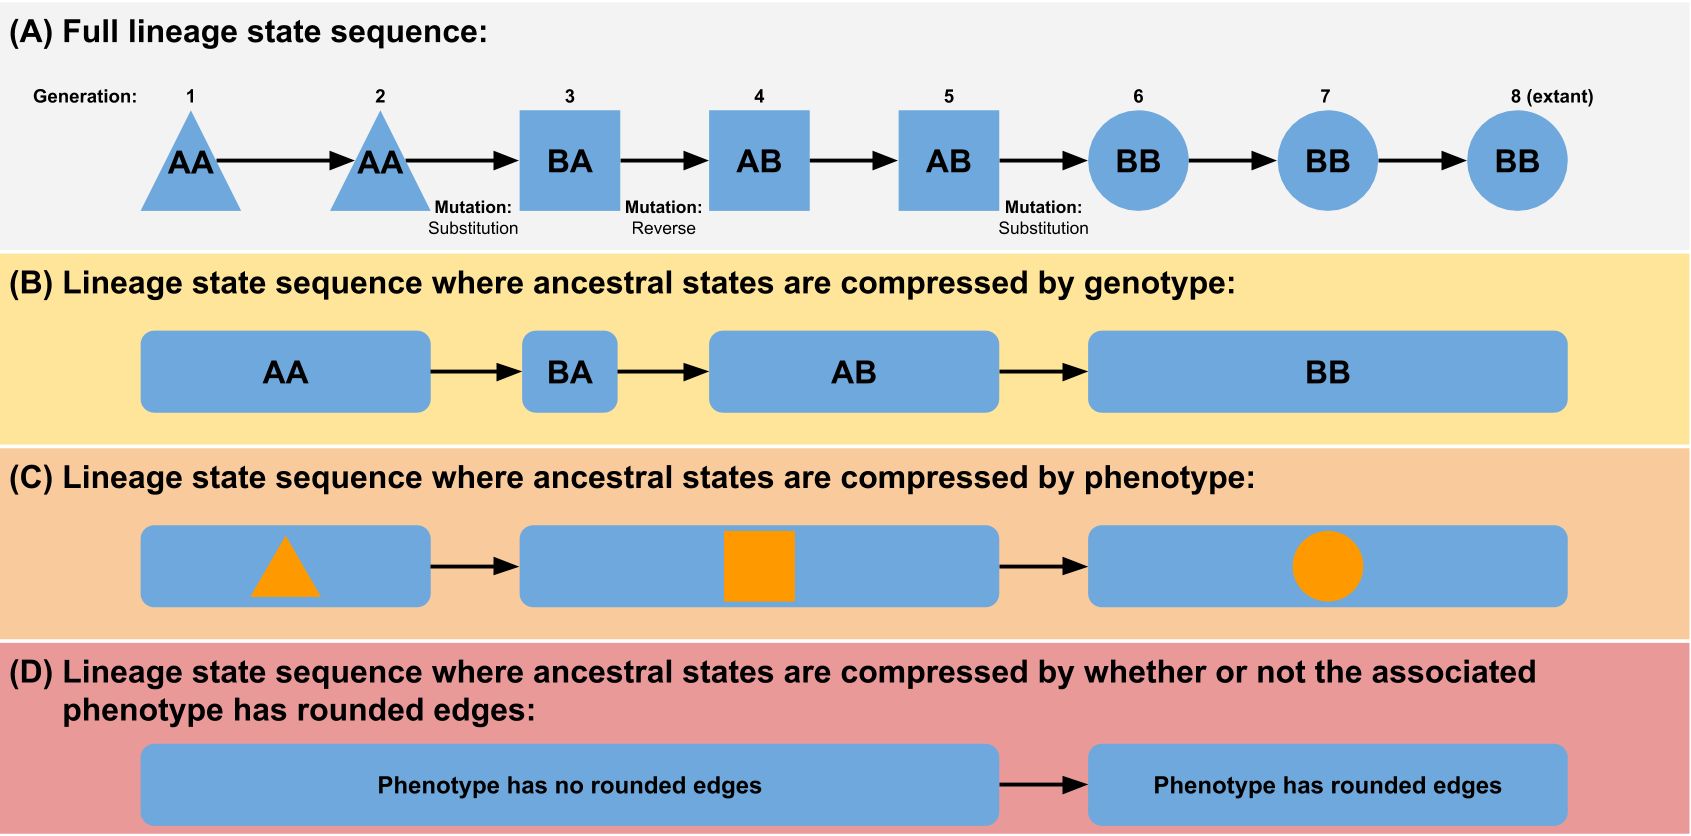
\includegraphics[width=\textwidth]{figs/lineage_metrics_cartoon.png}
\reduceCaptionPadding
\caption{\small Four methods of representing a lineage.  This example lineage has accumulated three mutations (one reverse mutation and two substitutions) and gone through three distinct phenotypes. In (A), each state along the lineage represents a single individual; lineage length is the number of generations spanned by the lineage (eight). In (B), states represent the sequence of genotypes along the lineage, reducing lineage length to four. In (C) states represent the sequence of phenotypes along the lineage; lineage length is the number of times a different phenotype is expressed (three). In (D), states are a particular phenotypic characteristic; here, lineage length is two.}
\label{fig:lineage_metrics_cartoon}
\end{figure*}

Each of the three lineage metrics that we discuss --- lineage length, mutation accumulation, and phenotypic volatility --- reduces a lineage to a linear sequence of states where each state represents an individual or sequence of individuals that share a common genotypic or phenotypic characteristic of interest; Figure \ref{fig:lineage_metrics_cartoon} is given as a toy example to help guide our discussion of these metrics. 
While we limit our focus to three lineage metrics, this abstraction places lineages in a form suitable for a wide range of measurements, including the direct application of many data mining techniques designed to operate over sequences such as sequential pattern mining, trend analysis, \textit{et cetera} \citep{han2011data}. 

Only asexual lineages %consisting of asexually reproducing ancestors 
where genetic material is exclusively vertically transmitted can be directly abstracted as a \textit{linear sequence} of states.
Sexual reproduction (and any form of horizontal gene transfer) complicates matters significantly as such lineages are more appropriately represented by trees rooted at the extant organism, branching for each contributor of genetic material. 
% For the metrics we present here, we limit our discussion to asexual populations; however, we suggest two approaches for generalizing these lineage metrics to sexual populations: apply a lossy compression to reduce sexual lineages into linear sequences or extend our application of the metrics to operate over non-linear (tree) structured lineages. 
One possibility is to compress sexual lineages into linear sequences of states by modeling sexual reproduction events as asexual reproduction events, designating one parent to be a part of the lineage and considering the genetic contributions of other parents as sources of genetic variation (mutations). The primary downside to this approach is its lossy-ness (\textit{i.e.}, the fact that it discards potentially important parentage information). 
Alternatively, we can extend our metrics to operate over the more complex state sequences that constitute the lineages of sexually reproducing organisms. One such approach would be to consider all possible ancestor paths for an extant individual, calculating a given metric for each of them and then averaging the resulting values together. Another approach would be to divide an organism into its constituent parts that are inherited atomically (such as genes or instructions, depending on the representation); an organism would then be viewed as a collection of lineages rather than a single one. 
Assessing the efficacy of these and potentially other approaches would be a useful line of research to pursue in the future.

\subsubsection{Lineage Length}
Lineage length describes the number of states traversed by a lineage. If a state is defined as a single individual, %along a lineage,
lineage length is a count of the number of generations.
%on a lineage.
%This form of the lineage length metric 
Generation count is most useful in systems where generational turnover is not fixed, %algorithmically determined,
but instead determined by the life history strategies of organisms.
%In these systems, %lineage length can provide a proxy for replication rate where, 
For lineages that span equal lengths of time, more generations imply faster replication rates (\textit{e.g.}, r-selected lineage) while fewer generations imply slower replication rates (\textit{e.g.}, K-selected lineage). 
%@ELD: I've always heard these called r- and k- selected rather than replicator, but I'm totally willing to believe these terms are used too.
%@AML: Yup. I have no idea if I've ever heard them referred to as 'r-replicator vs. k-replicator'. I'm going to get rid of the two parentheticals for now.
%@ELD: I like the idea of putting it in that context. I was just suggesting we replace "replicator" with "selected"
%@AML: Put the parentheticals back. 

Lineage length becomes %an increasingly 
a more flexible and informative metric if we consider more abstract definitions of %an ancestral 
states along a lineage. 
We might measure lineage length where a state represents a %temporally continuous 
sequence of individuals that share a particular phenotypic or genotypic characteristic.
%of interest. 
In these cases, lineage length only increases when the characteristic of interest changes from parent to offspring. For example, in an environment where organisms must perform tasks to be successful, we might define state as the set of tasks performed by an individual. %(\textit{e.g.} the set of logic operations performed by a digital organism in the default logic-9 Avida environment).
In this scenario, lineage length would only increase when the set of tasks performed by an ancestor changes; sequential ancestors that perform the identical sets of tasks would be compressed into a single state in the sequence, even if other traits differ. 
% This could be made very clear with a good example here. 
%@ELD Maybe I'm just getting tired, but I didn't quite follow that last sentence
%@AML: It was definitely hard to follow. Hopefully it's better now?
%@ELD: That definitely helped. I tried tweaking it a little more (I think the term "ancestral state" was confusing me, because I'm used to it being the state of the ancestor at the root of the tree)
%  -- Still could use a sentence about what the measure might tell us in the given example. 

\subsubsection{Mutation Accumulation}
Mutation accumulation defines a set of measurements that track mutational changes across a lineage. These changes can be measured %in a variety of ways, such 
as the magnitude of the change (for real-valued genomes) or as the total count of changes (for discrete-valued genomes). Mutation effects can also be tracked to gain insights about their distribution along a given lineage. Measures of mutation accumulation along the lineages of successful individuals can help tease apart the relative importance of different types of mutational events when compared to what is expected by chance. 

In conjunction with collected fitness information, the class of a mutation (\textit{e.g.}, beneficial, deleterious, or neutral) can also be tracked. Different evolutionary conditions are expected to cause different distributions of mutations along a lineage~\citep{barrick2013genome}; deviations revealed by measures of mutation accumulation can act as a barometer for unexpected evolutionary dynamics.  
% @AML: the below points likely have many things that could be cited to support. 
The number and magnitude of deleterious mutations along a lineage can tell us both about the ruggedness of the fitness landscape, and about a lineage's ability to cross fitness valleys~\citep{covert_experiments_2013}. 
Similarly, an elevated measure of neutral mutations relative to beneficial or deleterious mutations can suggest that the fitness landscape has neutral space that the lineage is spending most of its time drifting around. 
%@CAO There are various other things it could tell us, such as additional co-evolutionary pressures that are not reflected in the raw calculation of fitness.  Interestingly, using these metrics in combinaton with local fitness landscape analyses would do the trick.  But that's for another paper.  Indeed, I think it would be nice to put out a series of papers of useful analysis techniques and then do a master paper that reviews them all and demonstrates them in the context of an Avida-like system AND a very different digital evolution system (Markov Brains?)


% Mutation accumulation over a lineage 
%  - Measured in a variety of ways
%   - For real-valued genomes, we can track magnitudes of changes
%   - For discrete-valued genomes, we can track counts of changes
%      - Track by type to get distribution of mutation types
%   - In conjunction with fitness information, can track classes of mutation: beneficial, deleterious, neutral
%      - Again, can extract a distribution; different environments/experiments, you might expect different distributions
%      - Importance of deleterious steps; valley crossing, etc

\subsubsection{Phenotypic Volatility}

Phenotypic volatility addresses the rate at which phenotype changes as you move down a lineage (although the same concept can be applied to specific phenotypic traits or other types of state). In systems with discrete/categorical phenotypes, this can be measured by summing the number of times the phenotype changes. A related but subtly different measurement in such systems is the number of unique phenotypes on a lineage. In most cases, these values will be similar; a discrepancy
%between them, however, would be a clear signal of interesting dynamics. Specifically, it 
would suggest that the lineage was %in a portion of the landscape where it could rapidly switch among different 
cycling through a set of
phenotypes. Such behavior could, for example, be indicative of some form of evolutionary bet-hedging~\citep{beaumont2009experimental}. % @AML: There are a whole lot of citations for bet-hedging.. Just picked a popular Nature article on experimental evolution of bet hedging. Alternatively, could go with older paper suggesting bet-hedging as a possible strategy that exists. 
%@ELD: This one sounds good. Normally I'd say cite both, but we probably don't have the space.

In systems with continuous-valued phenotypes, a subtly different approach is needed to measure phenotypic volatility, because there are no discrete state transitions. Instead, we can measure the overall variance in phenotype along a lineage. In some cases, it may be desirable to smooth out the noise inherent in a real-valued phenotype. We can do so by instead taking the variance of the moving average of fitness, to more closely approximate the idea of measuring phase transitions.
% SPJ: What is meant by 'rolling mean' ?
%@ELD: Would "moving average" be more familiar? 
%@ELDL Also there turns out not to be much of a difference, so we could just not mention that approach.
% @SPJ: I don't think I have heard either of those terms. If we need space, it may be something to cut?
% @CAO: I suspect "moving average" is the more popular term, but I suspect people would figure out what we meant by either.
% @ELD: Okay, I changed it, but also this sentence is the first to go if we run into space issues.

% Define/describe
% .... 
% Useful things that this metric could identify:
% - Mutational bet hedging (high volatility)
% - Plasticity (high volatility)
% - Neutral landscapes (expect low volatility)

\subsubsection{Summary statistics}

Each of these metrics can be calculated for each member of the population at each time step. Doing so, however, would produce an amount of data so large that it would be difficult to make sense of. Instead, we need to come up with ways to generate useful summaries. There are two main approaches to doing so: 1) choose a small number of representative lineages from a given time point, or 2) collect summary statistics about the distribution of metric values across the population.

A single lineage can be chosen by selecting the lineage of a representative organism 
% OLD TEXT: (either the most fit or the most numerous; here we use the most fit). -- @AML: most fit in niching problems, most numerous in Avida
(either the most fit or the most numerous). 
In populations where diverse strategies coexist, this approach can be uninformative as any one lineage is unlikely to be representative of all successful lineages. One alternative is to filter out lineages that do not have offspring some predetermined number of generations later as such lineages were likely not representative of an important subset of the population. Still, any approach based on measuring only a subset of lineages can be challenging to interpret when the current dominant lineage (or lineages) is replaced with a different one; such changes can introduce a discontinuity if the value is being measured over time. If graceful responses to changes in which lineage is dominant are required, it can be advantageous to instead measure summary statistics (\textit{e.g.}, mean, variance, and range) across the entire population. 

In scenarios with frequent selective sweeps, the dominant lineage will likely be similar to the average lineage,
%in the population,
as most of the population will be closely related. When the population contains more phylogenetic diversity, however, %it is possible for 
the dominant lineage may differ from the mean. Of course, the nature of such differences is likely informative about the evolutionary dynamics occurring in the population. 
%Since we have yet to observe an instance of this phenomenon, we do not explore it further in this paper. 
% @AML: Not sure what the above sentence is saying.
%Nevertheless, it presents an argument for measuring the dominant lineage in addition to gathering summary statistics across the population. % @SPJ: I am not sure what argument this is referring to? The fact that there may or may not be a dominant lineage that differs from the mean?
%@ELD: The point was just that sometimes the dominant lineage is different from the mean and that probably matters but we're not going to talk about it. Since we're going to be short on space, I think we can just cut these lines.

\subsection{Phylogeny metrics}

These metrics operate on entire phylogenies rather than single lineages within a population, eliminating the need to identify a representative organism or lineage.
Because they use data from the entire population, phylogeny metrics can be more computationally expensive to calculate than single lineage metrics. On the other hand, because most lineages tend to share substantial history, phylogeny metrics can usually be calculated more rapidly than full-population lineage metrics. %can be calculated across an entire population.
Note that phylogenies can be constructed with regard to any taxonomic level of organization, be it individual, genotype, phenotype, \textit{et cetera}. Thus, when we refer generally to items in a phylogeny, we will use the term \textit{taxa}.

A standard technique for saving memory and time when working with phylogenies in computational systems is to ``prune" them, removing 
%any taxa that are not either currently alive or the ancestor of taxa that are alive.
% either dead (extinct) branches, or ancestors common to the entire population.
%@CAO: (NEVERMIND - SIMPLIFYING FURTHER... Does the substition I made above make sense?  I'm not quite sure what was meant by "the ancestor of taxa that are alive".
dead (extinct) branches.
Since all of the phylogeny metrics we discuss here are borrowed from natural systems (where we do not have information about taxa without offspring), they all are designed to work on pruned phylogenies. Thus, for the remainder of this paper, we will assume we are working with pruned phylogenies.

In populations without ecological forces promoting coexistence, phylogenies should coalesce periodically, resulting in pruned lineages that mostly consist of a single path. When there is strong selection, this coalescence should happen even more rapidly. Thus, phylogenies with topologies that deviate from that expectation are an indication of ecological interactions within the population. The metrics discussed here can provide insight into the nature of those interactions and their long-term evolutionary effects. As a result, they are often referred to as phylogenetic diversity metrics~\citep{tucker_guide_2017}.

An important distinction between phylogenies in natural versus computational systems 
%to be aware of 
is that natural phylogenies are generally inferred from extant taxa, whereas computational phylogenies are directly recorded. %The inferred phylogenies used in natural systems 
Inferred phylogenies 
do not contain internal nodes except at branch points. They also do not contain history prior to the most recent common ancestor (MRCA) of all extant organisms. %in the extant population.
For consistency, we exclude pre-MRCA taxa from our analyses. However, we will not remove non-branching internal nodes, as these only serve to make our phylogenies more informative.

Here we provide a high-level summary of phylogeny metrics that we expect will be particularly useful. For more metrics and more detail on all of these metrics, see~\citep{winter_phylogenetic_2013, tucker_guide_2017}. 

\subsubsection{Depth of Most-Recent Common Ancestor}

The depth of the MRCA %(i.e. how many steps from the beginning of time did it occur?) 
(\textit{i.e.}, the number of steps it is from the original ancestor)
%is a useful metric because of the relatively high ratio of informativeness to ease of calculation.
is an informative metric and is easy to calculate.
A recent MRCA implies frequent selective sweeps and less long-term stable coexistence between clades. %The depth of the MRCA is easily calculated because most implementations of phylogeny pruning require keeping track of it already. 
Measuring the frequency with which the MRCA changes (\textit{i.e.}, the number of coalescence events) can also be informative, as some conditions can inflate the length of the lineage relative to other conditions without actually increasing the frequency of selective sweeps. This scenario is particularly likely when the population size is changing over time. A downside to the depth of MRCA as a metric is that any population that does have a stable ecology will likely never change its MRCA after the very beginning of evolution %(which is informative as a way of detecting stably coexisting branches in the phylogeny).
(which at least allows us to detect stable coexistence in the population).

\subsubsection{Phylogenetic Richness}

Measurements of phylogenetic richness quantify the total amount of evolutionary history contained in a set of taxa. The most traditional metric of phylogenetic richness is
%the one simply titled
``Phylogenetic Diversity", which is calculated as the number of nodes in the minimum spanning tree from the MRCA to all extant taxa~\citep{faith_conservation_1992}. Another approach is to calculate the pairwise distances between all taxa and sum them~\citep{tucker_guide_2017}. A third approach is to sum evolutionary distinctiveness, a measurement of a taxon's evolutionary uniqueness~\citep{isaac_mammals_2007}, across all extant taxa~\citep{tucker_guide_2017}.

\subsubsection{Phylogenetic Divergence}

Measurements of phylogenetic divergence quantify how distinct the taxa in the population are from each other and are often %the means of values that can be calculated for
averaged across
individual taxa. For example, one option is to 
%calculate the mean of the pairwise distances between 
average the pairwise distances across
all taxa in the population~\citep{webb_exploring_2000}. Similarly, phylogenetic divergence can be calculated by 
%calculating the evolutionary distinctiveness of each taxon in the population (as alluded to in the previous section) and taking the average of these values.
% @CAO: "can be calculated by calulating" ?
% @ELD: hah, oops.
averaging the evolutionary distinctiveness across each taxon in the population.
%(as alluded to in the previous section).

\subsubsection{Phylogenetic Regularity}

Measurements of phylogenetic regularity quantify how balanced the branches are in a phylogeny and are often the variances of values calculated for individual taxa. Just as the mean of the pairwise distances between all taxa in the population is a measurement of phylogenetic divergence, taking their variance is a measurement of phylogenetic regularity. The same is true of the variance of evolutionary distinctiveness across the population.

\section{Methods}

We applied the metrics defined above to four benchmark functions from the GECCO Competition on Niching Methods \citep{li_benchmark_2013} and to four qualitatively different environments in the Avida Digital Evolution Platform.
Both of these evolutionary contexts are well understood and studied, making them particularly well suited for building our intuitions about what our proposed suite of ancestry-based metrics can tell us about evolutionary dynamics.

\subsection{Niching Competition Benchmark Problems}

\begin{figure}
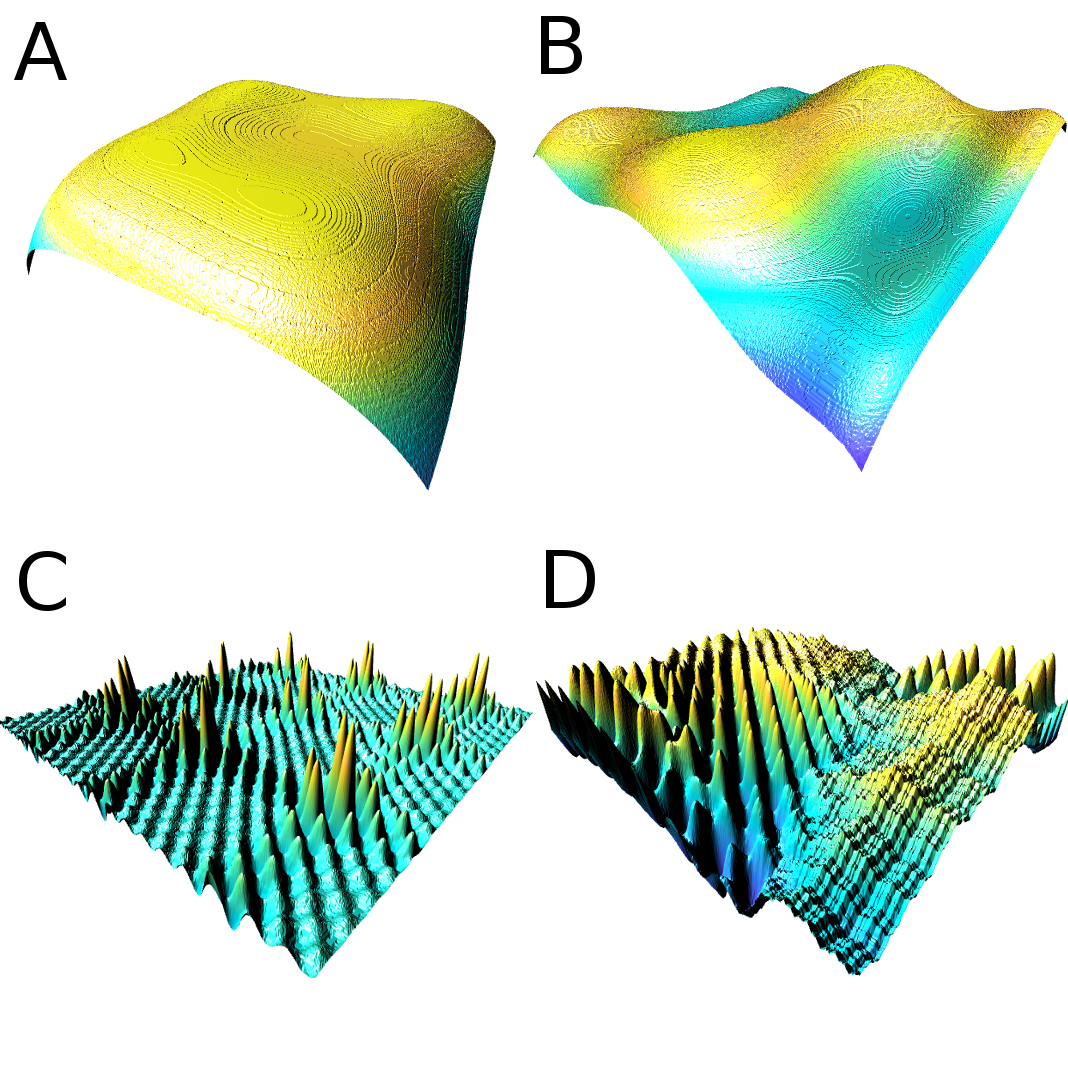
\includegraphics[width=\columnwidth]{figs/landscapes.png}
\reduceCaptionPadding
\caption{\small The fitness landscapes used in this experiment: A) Himmelblau, B) Six-humped Camel Back, C) Shubert, and D) Composition Function 2. Interactive versions available at \url{https://emilydolson.github.io/fitness_landscape_visualizations}.}
\label{fig:landscapes}
\end{figure}

To gain a broad understanding of our metrics, we applied them to a diverse subset of benchmark problems from the GECCO Competition on Niching Methods: Himmelblau, Shubert, Composition Function 2, and Six-Humped Camel Back~\citep{li_benchmark_2013}. For each test problem, the X and Y coordinates offered by a given organism are translated by the function into a fitness value. Because of their low dimensionality, we can fully visualize each problem's actual fitness landscape, allowing us to directly view how our ancestry-based metrics respond to the actual paths evolved lineages take through the fitness landscape under different conditions.
We used the implementations of these problems at \url{https://github.com/mikeagn/CEC2013} (C++ for fitness calculations during evolution, Python for post-hoc analysis). Figure \ref{fig:landscapes} shows the fitness landscapes defined by each of our four chosen test problems.

For each test problem, we evolved populations of 1000 organisms under a range of mutation rates and selection strengths for 5000 generations. Each organism's genome consisted of two floating point numbers that defined its position in the fitness landscape.
We initialized populations by randomly generating a number of organisms equal to the population size.
To determine which orgniams reproduced each generation, we used tournament selection. We evolved populations under five different tournament sizes: one, two, four, eight, and sixteen. Tournament size represents strength of selection where higher tournament sizes correspond to strong selection and lower tournament sizes correspond to weak selection~\citep{blickle1995mathematical}.
A tournament size of one is equivalent to no selection pressure (\textit{i.e.}, every organism in the population has an equal chance of being selected to reproduce). Organisms selected to reproduce did so asexually. Values in an offspring's genome were mutated by adding noise given by a normal distribution with a mean of 0; the `mutation rate' of a treatment defined the standard deviation used to define this normal distribution and was given as a proportion of the test problem's domain. 
We prevented mutations from causing a value to exceed the valid domain of the given problem. 
For each problem and tournament size, we evolved populations at eight mutation rates: $1\text{e-}08$, $1\text{e-}07$, $1\text{e-}06$, $1\text{e-}05$, $1\text{e-}04$, $1\text{e-}03$, $1\text{e-}02$, and $1\text{e-}01$. 

We also ran a second set of experiments using these benchmark problems to explore the impact of ecological dynamics on our suite of ancestry-based metrics. For these experiments, we generated a stable ecology using the Eco-EA algorithm as a selection technique~\citep{goings_ecology-based_2012}. Eco-EA is %essentially 
a technique for creating niches that promote stable diversification in the context of an evolutionary algorithm. In %the context of 
our test problems, we created niches associated with spatial locations across the fitness landscape. 
For all experimental conditions, we ran ten replicates, each with a unique random number seed. 
Our experiment is implemented using the Empirical library; our implementation is included in the supplemental material for this paper \citep{supplement}. 

\subsection{Avida}

% @AML: For our results/experiment, the fact that we're using Avida isn't all that important, so this section may be too detailed. If we don't have space, I could see trimming this quite a bit and outsourcing more of the details of how Avida works to citations.

% @AML: Image of the virtual hardware? Probably not necessary, but if we end up having extra space, why not?

The Avida Digital Evolution Platform \citep{ofria_avida:_2004} is a well-established artificial life system that has been used to study a wide range of evolutionary dynamics such as [examples with CITATIONS].
Avida's track record and popularity make it a good next step in testing our intuitions for how our suite of lineage and phylogeny metrics will respond under a range of evolutionary dynamics.
% @AML: might also want to mention how fitness landscapes are drastically more complex and more realistic relative to the niching benchmark problems.

In Avida, populations of self-replicating digital organisms compete for space in a finite, toroidal grid. 
Each digital organism has a set of virtual hardware and a circular genome composed of assembly-language-like instructions.
An organism's virtual hardware contains components such as a central processing unit (CPU) for executing instructions, registers used for computation, memory stacks, and input and output buffers. 
The instruction set of Avida is Turing-Complete and enables organisms to perform basic computations, control their own execution flow, and replicate. 
Further, the Avida instruction set is syntactically robust --- all possible genetic sequences are syntactically valid, even if they do not perform a meaningful computation.

Organisms in Avida replicate asexually by copying themselves instruction-by-instruction and dividing; copy and divide operations, however, are not perfect and can result in mutated offspring.
When an organism successfully replicates, the resulting offspring is placed randomly in the world, replacing that location's former occupant.
Thus, there is selection pressure for organisms to replicate quickly before being copied over by others.

A digital organism's replication speed can be improved by reducing the amount of instruction executions required for an organism to copy itself (\textit{e.g.}, by optimizing the self-copy genetic machinery) or by increasing its metabolic rate. Metabolic rate determines the speed at which an organism executes instructions in their genome; a higher metabolic rate allows an organism to execute its genome faster, which, in turn, allows the organism to copy itself faster. 
Initially, an organism's metabolic rate is approximately proportional
to its genome length; however, organisms can influence their metabolic rate by performing particular tasks, such as mathematical computations.
In this way, we can differentially reward or punish the performance of different computational tasks.
% @AML: Do we want to talk in terms of resources here or only bring them up when talking about the limited resource environment?

% todo - clarify hyphen in Bugs in Writing book
We evolved thirty replicate populations of size 500 in four different environments: a no-task environment, the logic-9 environment, a limited resource environment, and a simple changing environment. %With the exception of the limited resource environment, 
% - [insert some overarching justification for different environments, contrast with benchmark problems - richer dynamics, more complex genotype-phenotype mapping, implicit selection, life history traits, etc].
% - Insert relevant experiment parameters that are generic across treatments


% ENVIRONMENT: minimal - describe, intuitions w/respect to metrics
In the \textbf{no-task environment}, we did not reward any computational tasks. Because these digital organisms cannot influence their execution speed by performing computational tasks, selection pressure is entirely focused on optimizing the efficiency at which organisms can self-replicate. 
Thus, we expected lineages with short generation times to be most successful, resulting in long lineages comprising many individuals. This no-task environment has only a single niche, so we expected to see low phylogenetic diversity and frequent population-wide selective sweeps, each leading to a change in most recent common ancestor (MRCA).
% Todo - work in sentence comparing no-task environment to LTEE


% ENVIRONMENT: logic 9 - describe, intuitions w/respect to metrics
In the \textbf{logic-9 environment}, we rewarded the performance of all non-trivial one- and two-input Boolean logic functions: NAND, NOT, OR-NOT, AND, OR, AND-NOT, NOR, XOR, and EQUALS (for more information on these tasks in Avida see \citep{lenski_evolutionary_2003}). In addition to selection pressure for efficient self-replication, there is selection pressure for organisms to improve their instruction execution speed by performing logic functions. 
Logic-9, like the minimal environment, is a single-niche environment, so we expected to see low phylogentic diversity and frequent selective sweeps. However, because this environment rewards performing tasks, we expected to see lineages with longer generation times than those in the no-task environment. 
In addition to looking at individuals along a lineage, we compressed lineages into sequences of phenotypic task profiles. Each of the nine rewarded Boolean logic functions are of varying complexity to compute, NAND and NOT being the simplest and EQUALS being the most complex. Further, in the logic-9 environment, simpler tasks are building blocks for the more complex tasks. 
As such, we expected to see tasks appear on lineages in roughly the order of task complexity.
We can also use lineages compressed into sequences of task profiles to measure the rate of task acquisition (phenotypic volatility) or to look for trends in how long lineages spend in a particular phenotypic state, which can help untangle which phenotypic transitions might be the most challenging.


% ENVIRONMENT: limited resource - describe, intuitions w/respect to metrics
% @AML: Should we talk about inflow/outflow rates?
Like the logic-9 environment, the \textbf{limited resource environment} rewards the performance of all non-trivial one- and two-input Boolean logic functions; each of these computational functions, however, is associated with a limited pool of resources. When an organism performs one of the nine logic functions, it consumes resources associated with that particular function (lowering its concentration) in proportion to the resource's availability. 
Rather than adjusting organisms' execution speeds based directly on task performance, in the limited resource environment, an organism's execution speed is adjusted as a function of the amount of resources it has collected.
The limited resource environment has been shown to support stable ecologies via negative frequency-dependent selection \citep{cooper_evolution_2003}. 
Here, we expected the phylogeny metrics to reveal high phylogentic diversity relative to the other three environments. 
Because previous work has shown that the limited resource environment supports the stable coexistence of multiple ecotypes, we expect infrequent changes in the MRCA.

% ENVIRONMENT: changing - describe, intuitions w/respect to metrics
% - Description: alternatively reward and punish nand/not tasks
% - Cycling environment => Expect set of phenotypic states traversed by lineage to be low, but the total number of phenotype changes to be high
% - Expect rate of phenotype changes to approximate the environment change rate
%In the \textbf{changing environment}, populations were subjected to a cyclical, two-phase environment. 
In the \textbf{changing environment}, the rewarded functions cycled between 
%equal-length periods (200 updates* [explain updates, maybe in footnote]) of 
two opposing states: ENV-NAND (where we rewarded NAND and punished NOT) and ENV-NOT (where we rewarded NOT and punished NAND). 
ENV-NAND and ENV-NOT were configured such that no phenotype can be optimal across both environment states. To achieve maximal fitness in either ENV-NAND or ENV-NOT, organisms must perform \textit{only} the focal task.
In such environments, successful lineages should move to occupy a region of genotype space such that it is easier to mutationally toggle between a phenotype of only performing NAND and a phenotype of only performing NOT [CITE - some of Rose's work for this].
In this treatment, we expected to see a high number of phenotype changes but a low total number of unique phenotypes along evolved lineages.
Further, we expect the rate of phenotypic change along successful lineages to approach the rate of environmental change, as these lineages would have been more likely to produce offspring well adapted to the next environment.

% @AML: Need a sentence pointing out that specific configurations for all of these runs can be found in BLAH.


\subsection{Data Analysis}
\subsubsection{3D visualizations}

\begin{figure}
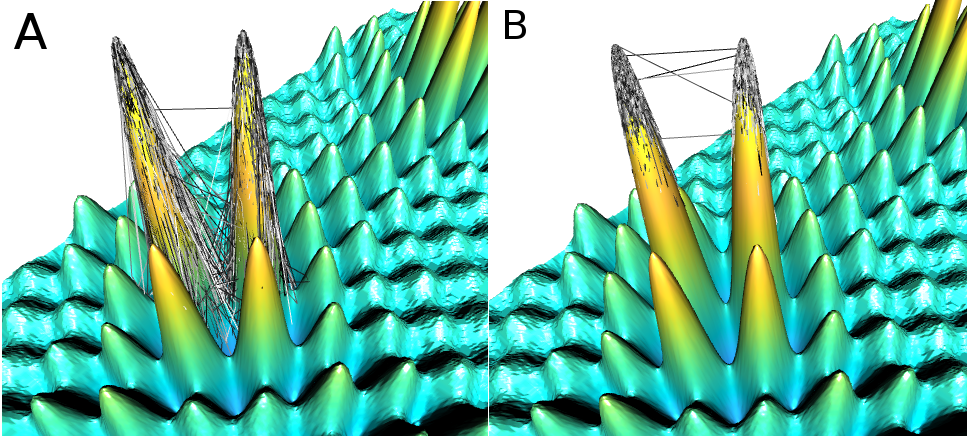
\includegraphics[width=\columnwidth]{figs/shubert_landscape.png}
\reduceCaptionPadding
\caption{\small A close-up on two adjacent peaks in the Shubert function fitness landscape. Lineages are depicted as paths fading from white to black over evolutionary time. The lineages shown here evolved under a mutation rate of 0.01. A) Was evolved using a tournament size of 2, whereas B) was evolved using a tournament size of 16. These figures neatly illustrate how increased tournament size keeps the lineage near the tops of the peaks.}
\label{fig:lineageviz}
\end{figure}


% Trim dramatically
%Evolutionary biologists often accuse each other of making up "just-so" stories - post-hoc explanations for how an observed trait or pattern could have evolved. The problem with these stories is that, in biology, there is often no way to verify that they reflect what happened in biology. Due to evolution's stochastic nature, it is easy to come up with possible ways that something could have happened once, regardless of how repeatable they are. Theoretically, we should easily be able to avoid this problem in computational evolution by carefully checking the underlying assumptions behind our hypothesized explanation.  All too often, however, we fail to drill down to the true underlying mechanism behind an observed effect.

%The metrics we propose here can help provide a check on this behavior, by making information about underlying evolutionary dynamics more readily accessible. They can only have that effect, however, if we completely understand what they are telling us about the way populations under different conditions are traversing different fitness landscapes. In order for these metrics to be useful for diagnosing the behavior of an evolving population, we need to establish ground truth for what underlying evolutionary dynamics are implied by different values of the metrics. For the purposes of building this intuition on a solid foundation, we wanted to be able to visualize the full evolutionary history of each population as it traversed the fitness landscape.

%To this end, we chose problems for which we could perfectly visualize the fitness landscape, and kept track of the complete evolutionary history of all members of the population. With these data, we were able to overlay successful lineages on top of the fitness landscape. Visualizing all lineages in each experimental condition in this way gave us an efficient check on our understanding of the underlying evolutionary dynamics in that condition. 
In order to make these metrics useful,
%in the long run, it is critical that 
we must have an accurate understanding of how various measurements correspond to the actual behavior of lineages. The most direct way to confirm our expectations is to visualize the path that each lineage takes through the fitness landscape, mapping the x, y, and z (fitness) coordinates of each ancestor of each member of the population~\citep{virgo_lineage_2017}. Creating such a visualization entails condensing a large quantity of information into a limited space. When projected onto two dimensions, lineages can obscure parts of the fitness landscape (and each other). To mitigate this problem, we used the A-Frame framework \citep{aframe} to build a three-dimensional data visualization (see Figure \ref{fig:lineageviz}) described in detail in our companion paper \citep{dolson_visualizing_2018}.
%A-Frame supports building %three dimensional 
%3D scenes and rendering them to a variety of platforms. In the simplest case, the visualization is rendered in WebGL, allowing it to be viewed in a standard web browser. Mouse interactions such as rotation make it possible to view the visualization from all angles, and WebGL's use of the graphics card allows it to render data-rich visualizations. A-Frame also supports rendering the page with WebVR, allowing it to be viewed using various virtual reality headsets. These platforms allow the user to explore the data in %a truly three-dimensional environment. 
%three dimensions.
%Different headsets support different amounts of interaction.
For the data interpretation in this paper, we used an Oculus Rift to provide us with fine-grained control of which part of the visualization we were looking at. Our full visualization, complete with data, can be viewed on the web or using a virtual reality headset at \url{https://emilydolson.github.io/fitness_landscape_visualizations}.

\subsubsection{POSSIBLE SUB-SECTION: Lineage Visualizations}

[To do]

\subsubsection{Metric analysis}

We analyzed trends in our metrics using the R Statistical Computing Language~\citep{r_core_team_r:_2017}. Specifically, we used the ggplot2 library for all graphs included in this paper~\citep{wickham_ggplot2:_2009}. All analysis scripts are available in the supplemental material for this paper \citep{supplement}..


\section{Results and Discussion}

\subsection{Niching Competition Benchmark Problems}

\begin{figure}
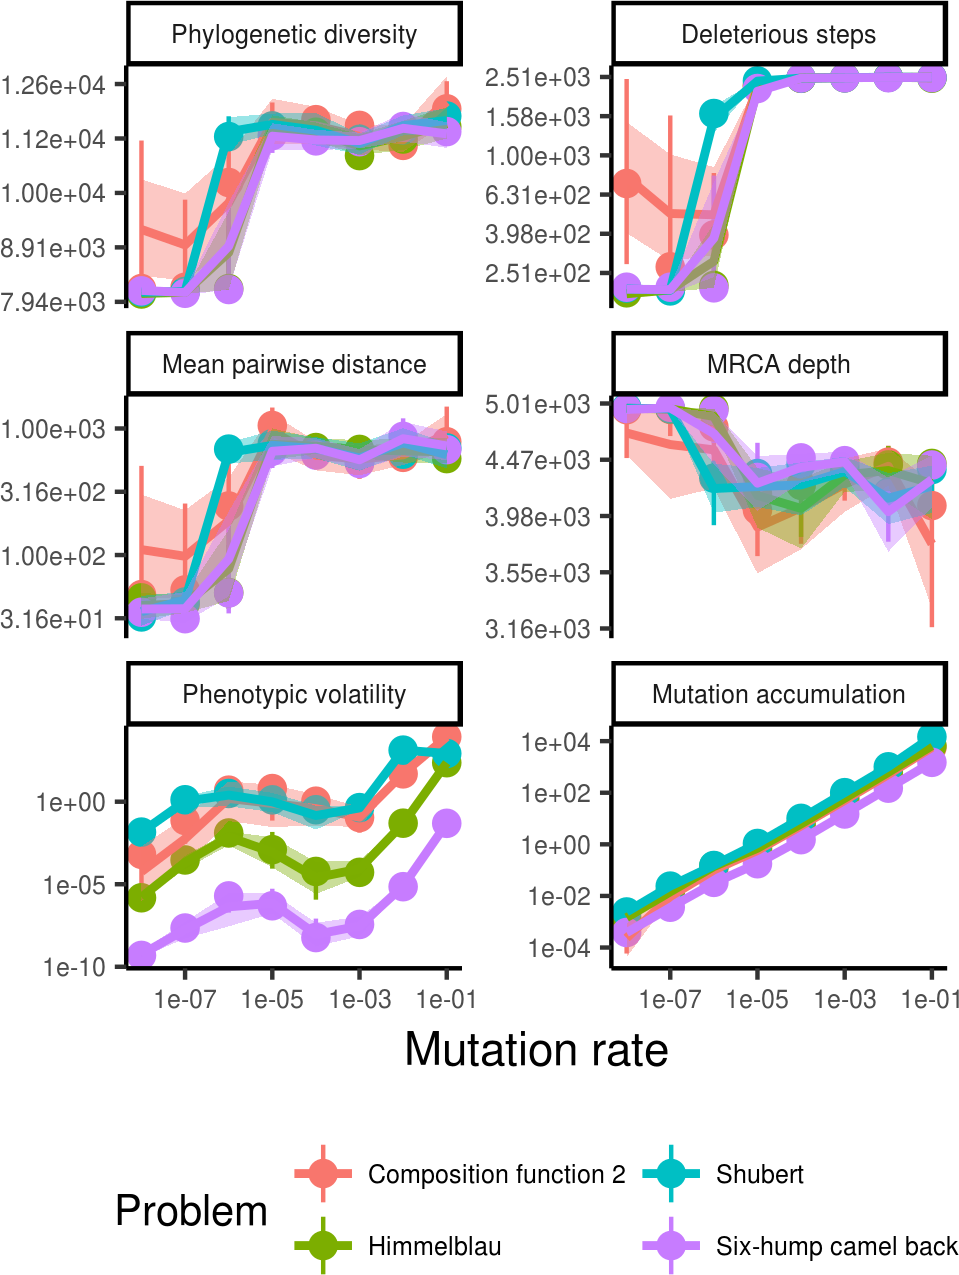
\includegraphics[width=\columnwidth]{figs/all_mutation_rate_crop.png}
\reduceCaptionPadding
\caption{\small Values of example metrics across different mutation rates for each of the four problems. All lineage-based metrics are calculated on the lineage of the fittest organism at the final time point; %(the dominant);
population-level means behaved similarly. All experiments shown here used a tournament size of 4. Circles are medians, vertical lines show inter-quartile range, and shaded area is a bootstrapped 95\% confidence interval around the mean. Note that both axes are on log scales.}
\label{fig:mutation_rate}
\end{figure}


Overall, our results were consistent with %what
evolutionary theory. %would predict. 
As mutation rate increases, coalescence takes longer, as evidenced by the fact that the MRCA is farther back in time at higher mutation rates (see Figure \ref{fig:mutation_rate}). Consequently, phylogenetic richness (as measured by phylogenetic diversity) is higher at high mutation rates. Phylogenetic divergence, measured here as mean pairwise distance between taxa, is similarly higher at high mutation rates. Evolutionary distinctiveness, being another measurement of phylogenetic divergence, behaved almost identically \citep{supplement}. Variance of evolutionary distinctiveness and pairwise distance between taxa (phylogenetic regularity metrics) behaved similarly to the phylogenetic divergence metrics. This pattern makes sense, as most phylogenetic divergence on these landscapes will produce unbalanced phylogenetic trees. If there were stable coexistence between multiple clades, we would expect to see a reduced correlation between the phylogenetic divergence metrics and the phylogenetic regularity metrics. Increased mutation rate also increases the number of deleterious steps taken, a logical consequence of increasing mutation relative to strength of selection.

\begin{figure}
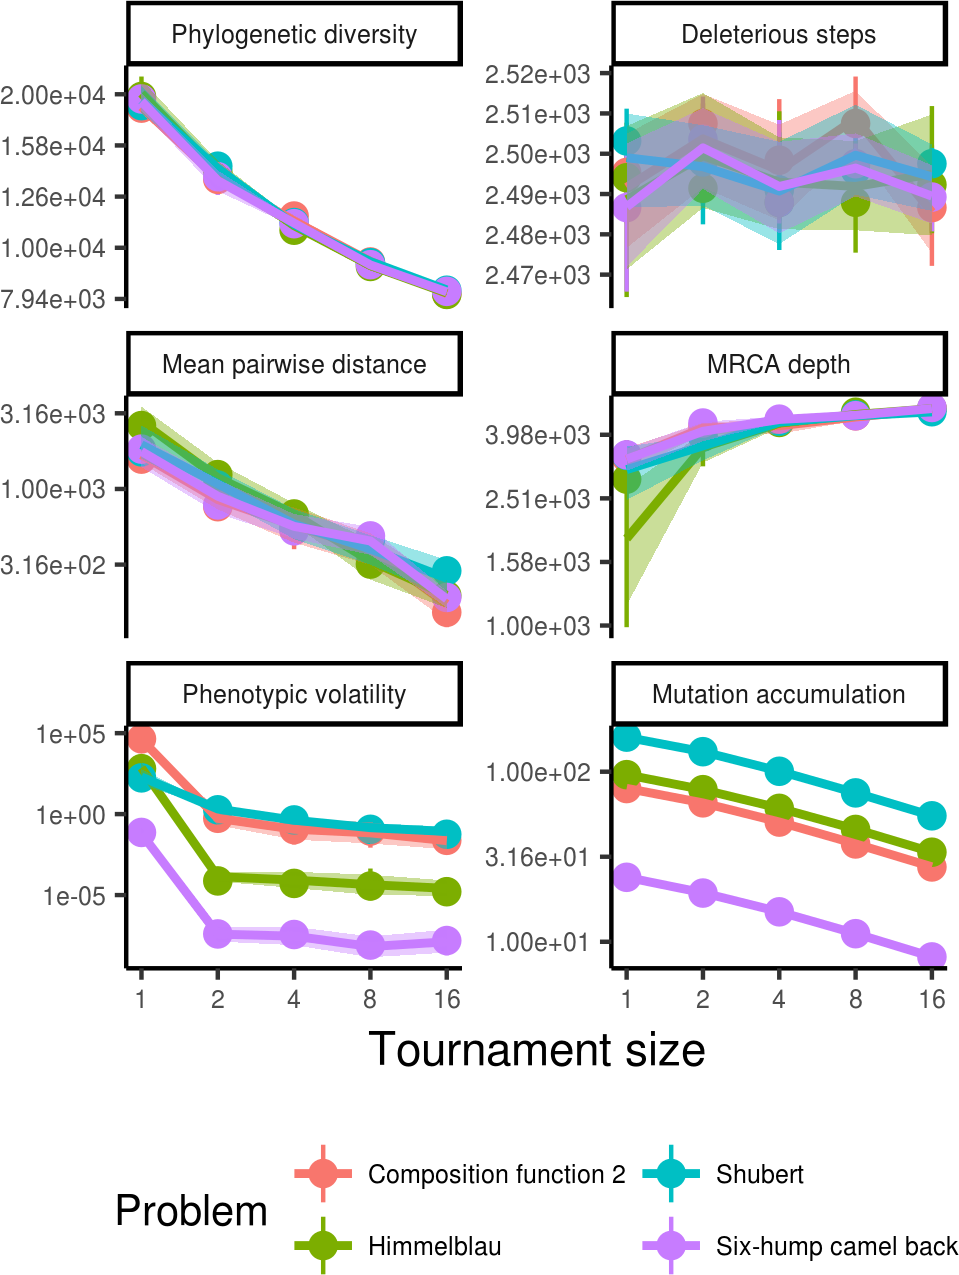
\includegraphics[width=\columnwidth]{figs/all_ts_crop.png}
\reduceCaptionPadding
\caption{\small Values of example metrics across different tournament sizes for each of the four problems. All experiments shown here used a mutation rate of 0.001. All lineage-based metrics are calculated on the lineage of the fittest organism at the final time point; population-level means behaved similarly. Circles are medians, vertical lines show inter-quartile range, and shaded area is a bootstrapped 95\% confidence interval around the mean. Note that both axes are on log scales.}
\label{fig:ts}
\end{figure}

Similarly, increasing tournament size generally increases the rate of coalescence, as higher tournament sizes correspond to stronger selection (see Figure \ref{fig:ts}). As a result, all of the measurements of phylogenetic richness and divergence decrease as tournament size increases. MRCA depth, on the other hand, increases, directly reflecting the increased frequency of selective sweeps. 

\begin{figure}
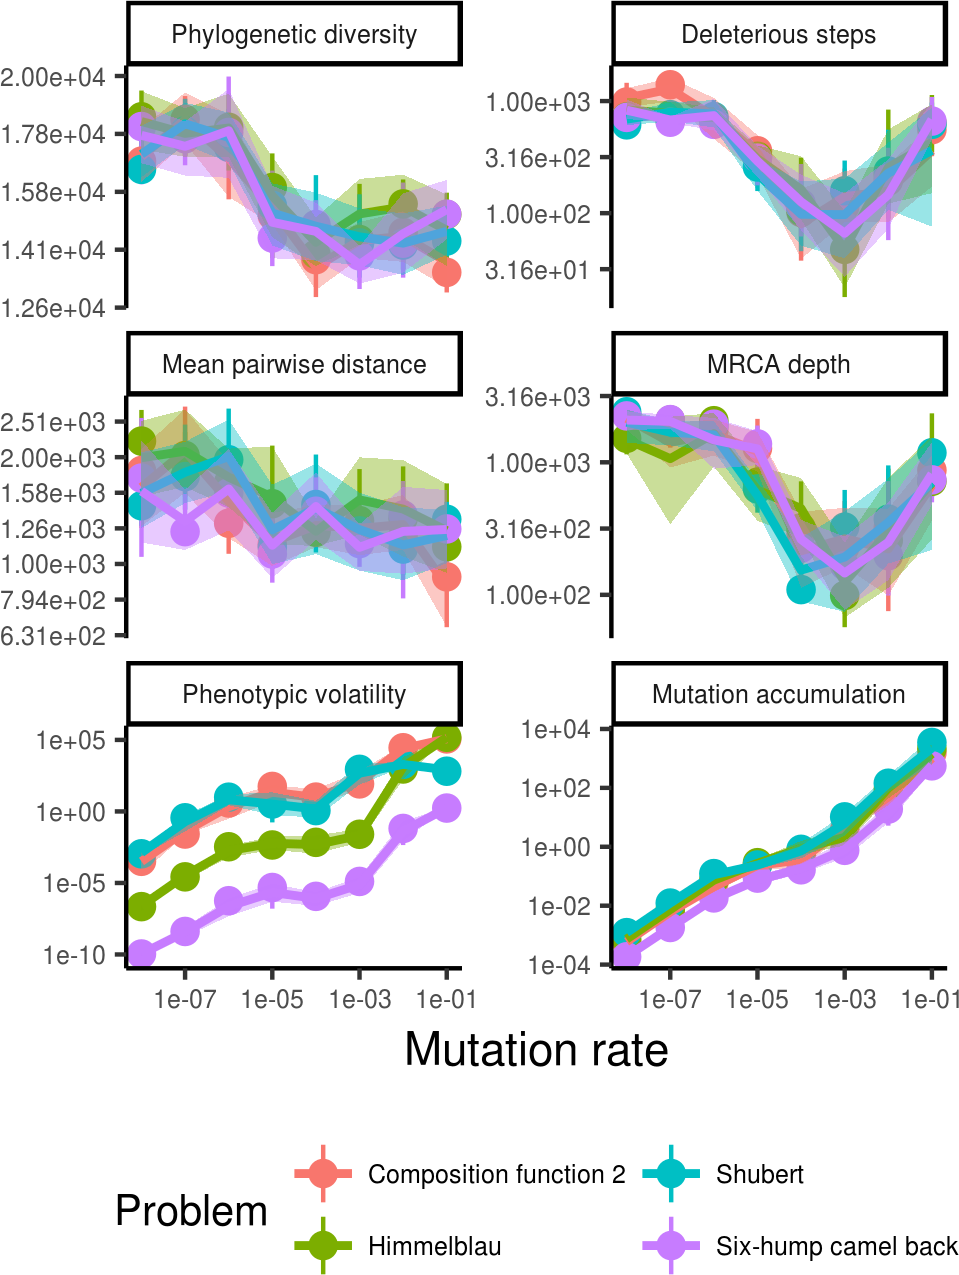
\includegraphics[width=\columnwidth]{figs/eco_mutation_rate_crop.png}
\reduceCaptionPadding
\caption{\small Values of example metrics across different mutation rates for each of the four problems under a diversity-preserving selection regime, Eco-EA. All lineage-based metrics are calculated on the lineage of the fittest organism at the final time point; population-level means behaved similarly. All experiments shown here used a tournament size of 4. Circles are medians, vertical lines show inter-quartile range, and shaded area is a bootstrapped 95\% confidence interval around the mean. Note that both axes are on log scales.}
\label{fig:ecology}
\end{figure}


Surprisingly, there is no clear effect of tournament size on the count of deleterious steps along the dominant lineage (as evidenced by the fact that the confidence intervals all overlap). Values for all selection schemes and tournament sizes hover near 2500, meaning that a deleterious step is taken in roughly half of the 5000 generations. This result is partially an effect of mutation rate; at the lowest mutation rate, there is a clear trend toward fewer deleterious steps as tournament sizes increase \citep{supplement}. However, the effect of mutation rate on the relationship between tournament size and dominant deleterious steps is complex, particularly for Composition Function 2 \citep{supplement}. These trends likely share a common cause with the thresholding effect evident in Figure \ref{fig:mutation_rate}, where the number of deleterious steps along the dominant lineage abruptly climbs between mutation rates of %0.0000001 and 0.00001 
$10^{-7}$ and $10^{-5}$
and remains relatively flat over other mutation rates. Based on an inspection of the %3-dimensional 
3D fitness landscape visualizations, we can see that this is not an effect of lineages moving from peak-to-peak; at most mutation rates, they tend to remain on a single peak. Thus, we can infer that this effect is the result of a drift-like phenomenon where, at sufficiently high mutation rates, all members of the population are constantly somewhat displaced from their local fitness peak.

Having %established that
reinforced our intuition about these metrics 
%are reasonable
in a simple system, we can now expand them to a slightly more complex system. A large proportion of interesting short-term evolutionary dynamics relate to interaction between individuals in the population (\textit{i.e.}, ecological dynamics). In particular, such interactions often promote the stable coexistence of clades occupying different niches. As such, it is important to establish a baseline for how our metrics respond to ecological coexistence. 

Indeed, the presence of stabilizing ecological dynamics substantially changes the values we observe for most metrics (see Figure~\ref{fig:ecology}). Perhaps the least surprising of these is MRCA depth is far lower than it was for tournament selection, reflecting the rarity of coalescence events under these conditions. Consequently, phylogenetic diversity is higher, as the extant population represents a greater amount of evolutionary history. Relatedly, mean pairwise distance among extant taxa is higher in the presence of ecology, as clades in different niches continue to diverge. Interestingly, the relationship of many metrics (\textit{e.g.}, deleterious steps and phylogenetic diversity) to mutation rate is reversed in the presence of ecology. Explaining the underlying mechanisms behind these distinctions is beyond the scope of this paper, but the ease with which the metrics identified their presence clearly indicates their power.

\subsection{Avida}


\section{Conclusions}

% Recap!
% In this work, we suggest a suite of lineage and phylogeny metrics aimed at improving our capacity to quantitatively understand observed evolutionary histories in digital evolution experiments. We applied these metrics to a set of toy problems, confirming theoretical expectations. 

Our goals for this work are two-fold: 1) to suggest a set of metrics that will improve our capacity to quantitatively understand evolutionary histories in digital evolution experiments, and 2) to spark a conversation in the computational evolution community about how to quantify, interpret, and compare observed evolutionary histories. With feedback from the community, we will expand our suite of lineage and phylogeny metrics, compiling accessible descriptions and examples of each metric. 

We have demonstrated that %the suite of lineage and phylogeny
these metrics behave reasonably on a set of toy problems with simple organisms. Having established baseline expectations for their responses to common conditions, our next step is to apply these metrics to more complex scenarios: populations of digital organisms that we evolve in a variety of qualitatively different environments where we would expect to observe a wide range of evolutionary dynamics. It is under these conditions that we expect the true value of these metrics to become clear.

\section{Acknowledgements}

% Extend thanks to:
%  - Devolab; thoughful discussions and whatnot
%@ELD: Anyone specific?

% Monies:
%  -  GRFP: Grants DGE-1424871
%   - NSF MT Grant: DEB-1655715. (for funds to develop Empirical tools)
%   - BEACON

% Other resources:
%   - MSU HPCC

We thank members of the MSU Digital Evolution Lab for helpful comments and suggestions on this manuscript. This research was supported by the National Science Foundation (NSF) through the BEACON Center (Cooperative Agreement DBI-0939454), Graduate Research Fellowships to ED and AL (Grant No. DGE-1424871), and NSF Grant No. DEB-1655715 to CO. Michigan State University provided computational resources through the Institute for Cyber-Enabled Research and the Digital Scholarship Lab. Any opinions, findings, and conclusions or recommendations expressed in this material are those of the author(s) and do not necessarily reflect the views of the NSF or MSU.

\setlength{\bibsep}{2pt}

\footnotesize
\bibliographystyle{apalike}
\bibliography{paper/Zotero,paper/bibliography} % replace by the name of your .bib file

\end{document}

% ===== Where old comments go to die:  ======

% Outlining some points to (maybe) make here; probably too bogged down in details; not even sure we want to talk about lineages as graphs:
% - Apply metrics in context of asexual populations
% - Establish a framework from which to think about metrics (not novel, but rarely formalized)
% 	 - We treat lineages as sequences of states where each state represents an individual and transitions between states represent parent-offspring relationships.
%      - More formally, lineages are directed acyclic graphs where internal nodes have in-degree = 1 (parent), out-degree = 1 (offspring). Original ancestor (in digital evolution, often seed of population) w/out-degree = 1. Extant individual w/in-degree = 1.
%      - Transitions specify relevant variation introduced into offspring (e.g. mutations)
%      - States specify relevant genotype and phenotype information (e.g. genome, location in space, behavior, etc) -- anything we might want to measure over a lineage
%      - Becomes more complicated with sexual populations, but we'll stick with asexual assumption for this. 
%  - Already, framework affords certain questions:
%     - How many individuals are along the lineage? 
%     - Total # and magnitude of mutations along lineage?
%     - Distribution of mutation types (ins vs. sub/beneficial vs. deleterious)?
%  - Further abstractions:
%      - Sequence of genotypes along lineage (where each genotype may represent multiple individuals)
%      - Sequence of phenotypes along lineage (where each phenotype may represent multiple individuals)
%      - Still further abstraction: sequence of a particular aspect of genotype (e.g. genetic marker)/phenotype (e.g. location) along lineage
%  - We discuss three classes of lineage metrics within this framework: lineage length, mutation accumulation, and phenotypic volatility. 
%  - For each, we discuss our intuition for what they can tell us (alone and in combination) about evolution. 

% Define/explanation
% 	- Within context of framework, lineage length is simply measure of number of states in the graph/sequence.
%   - What this means will depend on what states represent?
%       - number of individuals along lineage 
%             - More interesting in experiments where generations are not dictated by system, but rather by life history strategies of organisms
%             - Give you a diagnostic for replication rate (r vs. k strategy)
%      - number of genotypes along lineage
%            - length = 1: no mutations
%            - length = number of individuals: mutation in every replication
%            - Intuitively, should be higher at high mutation rates, lower at low mutation rates. 
%      - number of phenotypes along lineage
%            - low: evidence for static environment
%            - high: might be indicative of a changing environment or ecological interactions
%            - if number of genotypes is high, but number of phenotypes low, probably in a neutral fitness landscape
%      - various subsets of genotype/phenotype
%           - location in space (environment type): useful for looking at lineage through heterogeneous landscape
%           - change in particular phenotypic trait
%           - change in genetic markers
%           - Distributions of above two lengths can tell you useful things about drift, selection, etc.
